\documentclass[12pt,a4paper]{article}

\usepackage[T1]{fontenc}
\usepackage{amsmath, amssymb, amsfonts}
\usepackage[magyar]{babel}
\usepackage[utf8]{inputenc}
\usepackage{graphicx}
\usepackage{graphics}
\usepackage{mathtools}
\usepackage{epsfig}
\usepackage{epstopdf}
\usepackage{cite}
\usepackage{caption}
\usepackage{hyperref}
\usepackage[bottom=4cm]{geometry}
%\geometry{a4paper, portrait, margin=1in}

\title{\huge{Alkalmazott Fizikai Módszerek Laboratórium}\\ \vspace{20pt}
\textbf{Pásztázó elektronmikroszkópia}}

\author{\Large{\textsc{Csörnyei Géza}} \vspace{10pt}\\
	\textrm{Eötvös Loránd Tudományegyetem}\\
	\textrm{Fizikus MSc I}
	}
\date{}
%\lhead{}
\begin{document}
\addtolength{\voffset}{-1.0cm}
\addtolength{\textheight}{1.0cm}
\begin{titlepage}
\maketitle

\begin{figure}[!htb]
\centering

\includegraphics[scale=0.6]{eltecimer.jpg}
\end{figure}

\hfil \Large{'E' mérőcsoport}\hfil  \\
\vspace*{2pt}
\hfil \Large{\emph{Mérés dátuma:} 2019.11.08.}\hfil \\
\vspace*{2pt}
\hfil \hspace*{45pt} \Large{\emph{Mérés vezetője:} Kolonits Tamás}\hfil
\thispagestyle{empty}
\end{titlepage}


\section{Bevezető}
\hspace{10pt} Mérésünk során megismerkedtünk a pásztázó elektronmikroszkópia elméletének, valamint használatának alapjaival. A méréseink kiértékelése során egy ismert méretű kalibrációs rácsról készült felvétel segítségével meghatároztuk egy ismeretlen rács, illetve egy légy szemének méreteit.

\section{Méréshez használt eszközök}
\begin{itemize}
\item{Jeol JSM-25S típusú elektronmikroszkóp}
\item{Számítógép a mikroszkóppal történő mérés elvégzésére}
\end{itemize}

\section{Rövid elméleti összefoglaló}
\hspace*{10pt} Mérésünk során pásztázó elektronmikroszkópot használtunk, mely a nevéből látszó módon elektronokat használ a képalkotáshoz. A mikroszkóp katódjából kilépő elektronokat egy szabályozható erősségű elektromos tér gyorsítja a szükséges energiára. Az így felgyorsított elektronokat ezt követően ráfókuszáljuk a minta egy adott pontjára, ahol ennek következtében különböző termékek keletkeznek. Ezen termékek közül számunkra a szekunder és a visszaszóródott elektronok a legfontosabbak, a pásztázó elektronmikroszkópiában ezeket használjuk. A szekunder elektronok a minta nyaláb felőli oldalán megjelenő elektronok, melyek elsősorban a gyengén kötött, külső elektronhélyon elhelyezkedő elektronok, melyeket a nyaláb kiüt a helyükről és topologikus, azaz felületi információt tartalmaznak a mintáról. A visszaszórt elektronok a nyalábból rugalmasan és rugalmatlanul, nagy szögű szórást szenvedett részecskék. Ezen elektronok képalkotásra használhatók. Ezen elektronokat egy a mikroszkóban található Everhard--Thornley-detektor alakította mérhető jellé. Mérésünk során csak a szekunder elektronokat vizsgáltuk, melyek a lehetséges legjobb felbontást szolgáltatják. A jó felbontás mellett a szekunder elektronok az anyagi minőségben vett eltérések megjelenítésére is használhatók, ugyanis ezen képeken a kontraszt jelentősen függ a letapogatott anyag atomjainak rendszámától.\\
\hspace*{10pt} A mérés során a behelyezett mintát a mikroszkóp pontról pontra letapogatta, majd a létrejövő termékeket mérve modulálta a képernyő egyes pixeleinek intenzitását. Az így kapott kép rendkívül jó mélységélességgel rendelkezett, a SEM képeken a különböző mélységben elhelyezkedő mintarészletek egyazon képek élesek voltak. 
\newpage

\section{Mérés menete}
\hspace*{10pt} A mérés megkezdéséhez a legelső elvégzendő feladatunk a minta mikroszkópba történő behelyezése volt. A minták a méréshez előre el lettek készítve, így megfelelően meg lettek tisztítva, valamint a biológiai minták kellőképpen ki lettek szárítva (mely a minta vákuumba történő behelyezése miatt volt fontos), valamint a nem vezető minták be lettek vonva egy vékony vezető (például arany) réteggel. Kiválasztott mintát egy csipesz segítségével kivettük a tárolóedényből, majd behelyeztük a mintatartóba. A lehetséges szennyeződések elkerülése végett ezen lépéshez kesztyű viselése volt szükséges. A mintatartóba történő behelyezést követően beállítottuk a minta magasságát úgy, hogy a mintatartó tetejével egy szintben legyen a minta. A mintatartó ezt követően visszakerült a mikroszkópba, majd a tartószerkezetet ütközésig visszatoltuk.\\
\hspace*{10pt}  A vezérlőpanelen megnyomva az \emph{EVAC} gombot a mintát vákuum alá helyeztük, mely folyamathoz több percre is szükség volt. A vákuum létrejötte után be kellett állítanunk  a mikroszkóp optimális intenzitását. Optimális intenzitás esetén nem csak a rendszer munkapontját állítjuk be, de a katód élethosszát is megnöveljük. Ezen beállítást követően a kontrasztot (\emph{Contrast}) és a fényerőt (\emph{Brightness}) változtatva megkerestük a vizsgálni kívánt tartományt. A tartományon egy kicsi pontszerű objektumot keresve beállítottuk a rendszer fókuszát (\emph{Focus Coarse} és \emph{Focus Fine}), majd korrigáltuk a lencse asztigmatikus hibáját (\emph{Stigmator}). Ezt követően kisebbre állítottuk a nagyítást, majd felvettünk a kívánt tartományról egy képet, melyet a számítógépre továbbítottunk. A gépen látott fényerő és kontraszt nem egyezik meg a vezérlőpulton látottal, ezért a számítógép által számolt intenzitás hisztogramok segítségével a megfelelőre állítottuk ezen értékeket.\\
\hspace*{10pt} A képek elkészítése és a mérés elvégzése után levettük a katódról a feszültséget, majd lekapcsoltuk a gyorsítófeszültséget. A mikroszkóp alaphelyzetbe állításához megnyomtuk a \emph{VENT} gombot, mely hatására a mintatérbe levegőt engedtünk, majd kicserélhettük a mintát, a fentebb már ismertetett módon.

\section{Mérések kiértékelése}
\subsection{Kalibráció}
\hspace*{10pt} A kiértékelések elvégzéséhez meg kellett határoznunk az egyes ábrákon látható alakzatok valódi fizikai méreteit. Ehhez egy hatszögrácsokat tartalmazó réz mintát használtunk. A kalibrációhoz adott volt egy a mintáról készült kép, amelyen be voltak jelölve az egyes távolságok. A kép a \ref{fig:kalib}. ábrán látható. 
\begin{figure}[!h]
\centering 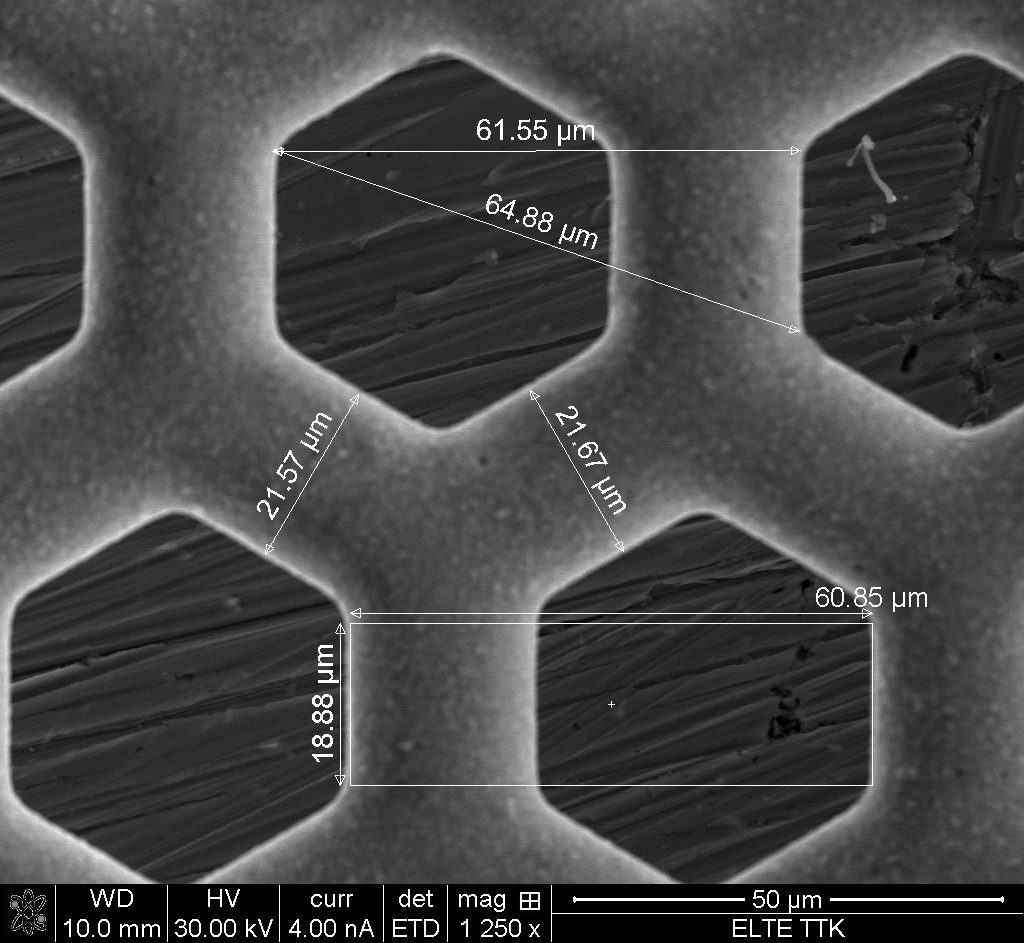
\includegraphics[width=0.8\linewidth]{E/kalib}
\caption{A kalibrációs rácsról  készült kép az egyes fizikai távolságokkal}
\label{fig:kalib}
\end{figure}

\begin{table}[!h]
\begin{center}
\hspace*{-0.7cm}
\begin{tabular}{|c|c|c|c|c|c|}
\hline
Nagyítás (x) & Fizikai méret [$\mu$m]& Méret a képen [px] & Kalibrációs faktor [$\mu$m/px] \\
\hline
150 & 61.55 & 63.03 & 0.977\\
\hline
150 & 64.88 & 66.85 & 0.970\\
\hline
150 & 21.57 & 23.26 & 0.927\\
\hline
150 & 18.88 & 21.01 & 0.899\\
\hline
300 & 61.55 & 130.14 & 0.473\\
\hline
300 & 64.88 & 139.46 & 0.465\\
\hline
300 & 21.57 & 47.51 & 0.454\\
\hline
300 & 18.88 & 44.05 & 0.429\\
\hline
700 & 61.55 & 296.20 & 0.208\\
\hline
700 & 64.88 & 314.38 & 0.206\\
\hline
700 & 21.57 & 109.13 & 0.198\\
\hline
700 & 18.88 & 104.08 & 0.181\\
\hline
1000 & 21.57 & 155.19 & 0.139\\
\hline
1000 & 18.88 & 139.01 & 0.136\\
\hline
2000 & 21.57 & 315.29 & 0.068\\
\hline
\end{tabular}
\caption{A készített képek vizsgálata során kapott értékek}
\label{tab:kalib}
\end{center}
\end{table}

\newpage

A táblázatban látható adatok segítségével kiszámoltam a kalibrációs faktor értékeket az egyes nagyítások esetére, melyet egyszerűen a kapott értékek átlagának tekintettem. Több mérés esetén lehetőségem volt a statisztikus hiba becslésére is, a kalibrációs faktorok szórásának számításával. Amennyiben ehhez nem volt elegendő mérés, ott a többi nagyítás esetén számolt relatív hibát alkalmaztam. A kalibrációhoz készített képek az oldal alján, valamint a következő oldalon láthatók.

\begin{table}[!h]
\begin{center}
\begin{tabular}{|c|c|c|}
\hline
Nagyítás (x) & Kalibrációs faktor [$\mu$m] & Hiba [$\mu$m]\\
\hline
150 & 0.943 & 0.032 \\
\hline
300 & 0.455 & 0.017 \\
\hline
700 & 0.198 & 0.011 \\
\hline
1000 & 0.138 & 0.002 \\
\hline
2000 & 0.068 & 0.002 \\
\hline
\end{tabular}
\caption{A számolt kalibrációs faktor értékek}
\label{tab:kalibs}
\end{center}
\end{table}

\begin{figure}[!h]
\begin{center}
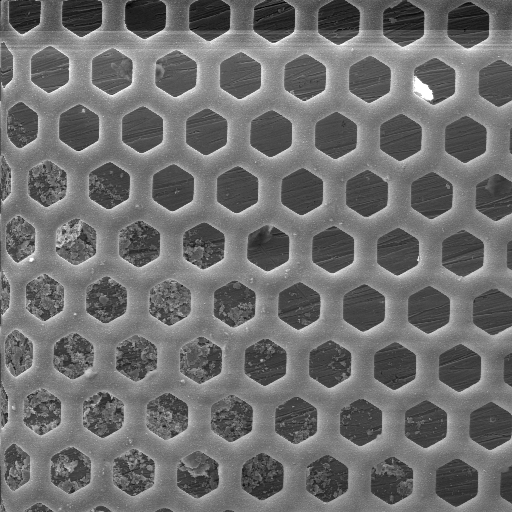
\includegraphics[width=0.45\linewidth]{E/E/008_s}
\hspace*{1cm}
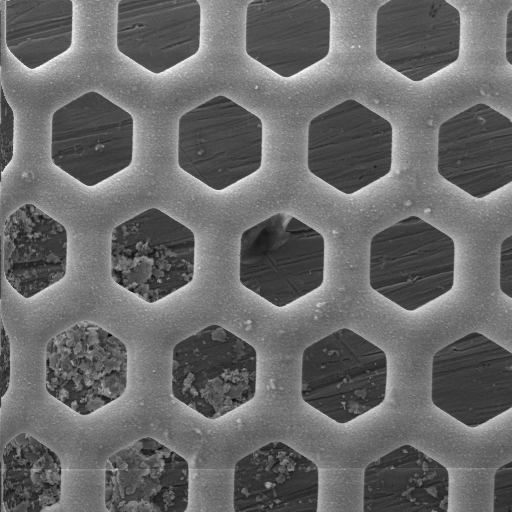
\includegraphics[width=0.45\linewidth]{E/E/009_s}
\caption{A kalibrációhoz használt képek, melyek a rézrácsról készültek. A bal panelen a 150x-es, a jobb panelen a 300x-os nagyítás mellett készült kalibrációs kép látható.}
\label{fig:kalibs}
\end{center}
\end{figure}

\newpage

\begin{figure}[!h]
\begin{center}
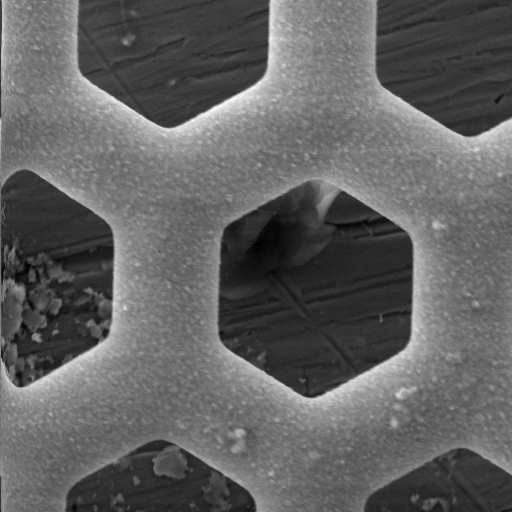
\includegraphics[width=0.45\linewidth]{E/E/010_s}
\hspace*{1cm}
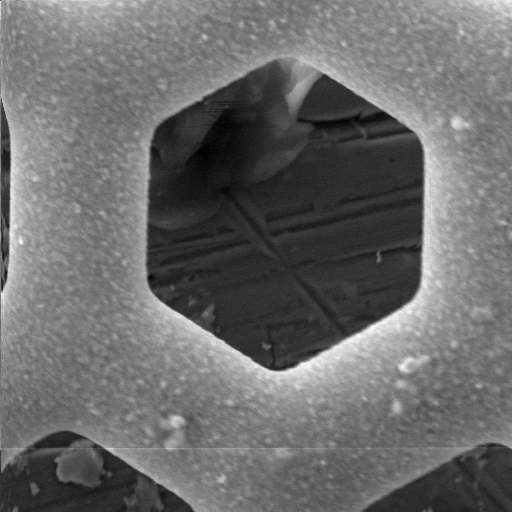
\includegraphics[width=0.45\linewidth]{E/E/011_s}
\caption{A kalibrációhoz használt képek, melyek a rézrácsról készültek. A bal panelen a 700x-os, a jobb panelen a 1000x-es nagyítás mellett készült kalibrációs kép látható.}
\end{center}
\end{figure}

\begin{figure}[!h]
\centering
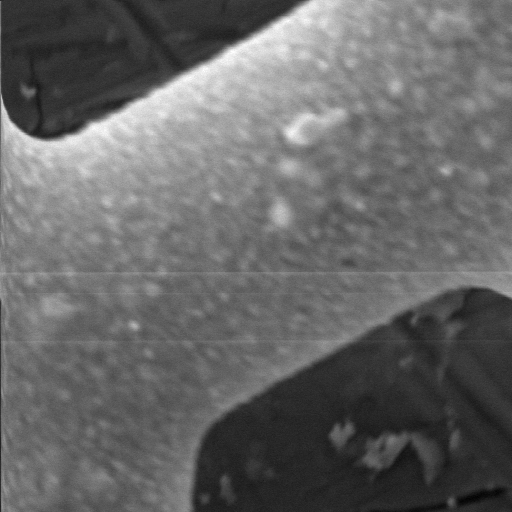
\includegraphics[width=0.45\linewidth]{E/E/012_s}
\caption{A kalibrációhoz használt 2000x-es nagyítás mellett készült kép.}
\end{figure}

\subsection{Szilícium minta mérésének kiértékelése}
\hspace*{10pt} A szilícium mintán mesterségesen kialakított mintázatok voltak láthatók, melyekre példa a \ref{fig:szil_pel}. ábrán látható. Feladatunk a mintán látható téglalapok területének megmérése, illetve ezen területek és a hozzájuk tartozó téglalapok mellett látható számok közötti kapcsolat elemzése volt. A nagyítás, a látható, valamint a kalibrációs faktorok segítségével számolt terület, valamint a téglalapok mellett látható számok a \ref{tab:szil}. táblázatban láthatók.
\newpage
\begin{figure}[!h]
\centering
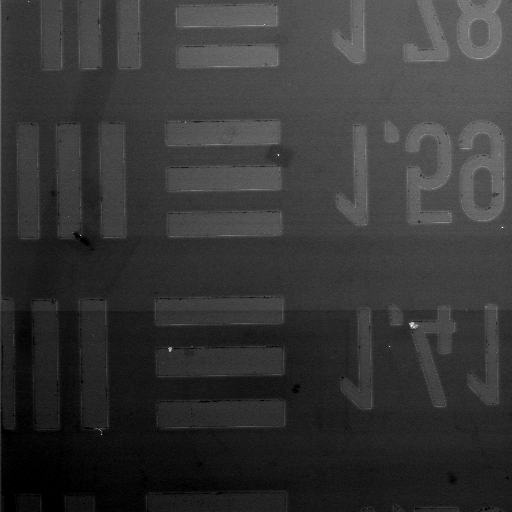
\includegraphics[width=0.6\linewidth]{E/E/002_s}
\caption{Példa a szilícium mintán látható mintázatra}
\label{fig:szil_pel}
\end{figure}

\begin{table}[!h]
\begin{center}
\hspace*{-1.5cm}
\begin{tabular}{|c|c|c|c|c|c|c|}
\hline
Sorszám & Nagyítás (x) & 1.terület (px) & 2. terület (px) & 3. terület (px) & Átlagos terület & Hiba\\
\hline
1.78 & 300 & 17945.00 & 18141.47 & 17784.72 &  17957.06 & 145.89\\
\hline
1.59 & 300 & 22450.00 & 22322.55 & 23052.14 & 22608.23 & 318.17\\
\hline
1.41 & 300 & 28589.53 & 30467.98 & 28730.51 & 29262.67 & 854.22\\
\hline
1.26 & 300 & 34608.34 & 34682.60 & 35276.25 & 34855.73 & 298.89\\
\hline
1.12 & 200 & 20610.00 & 20289.62 & 20229.00 & 20376.21 & 167.16\\
\hline
\end{tabular}
\caption{A szilícium minta képeiről leolvasott és számolt értékek}
\label{tab:szil}
\end{center}
\end{table}

A fent táblázatban összefoglalt értékeket át kellett váltani valós fizikai méretekké, melyet a kalibrációs faktorokkal tehettem meg. Minden átlagos értéket, valamint a hibákat megszoroztam a megfelelő kalibrációs faktorok négyzetével (mivel terület mennyiségekről van szó), majd a kapott értékeket a \ref{szil:ertek}. táblázatban foglaltam össze. A táblázatban látható hibákat a kalibrációs faktor hibájának és a területmérés statisztikus hibájából hibaterjedéssel számoltam.
\newpage
\begin{table}
\begin{center}
\begin{tabular}{|c|c|c|}
\hline
Sorszám & Terület [$\mu$m$^2$] & Hiba [$\mu$m$^2$] \\
\hline
1.78 & 3717.56 & 198.74\\
\hline
1.59 & 4680.47 & 255.93\\
\hline
1.41 & 6058.10 & 365.70\\
\hline
1.26 & 7216.01 & 386.27\\
\hline
1.12 & 9491.37 & 507.52\\
\hline
\end{tabular}
\caption{A számolt területértékek}
\label{szil:ertek}
\end{center}
\end{table}
Mivel a területek a sorszámok növekedésével csökkentek, valamint mivel látszólag nem lineáris csökkenésről volt szó, ezért a sorszámokkal fordítottan arányos függést tételeztem fel. Ennek fényben az illesztett függvény $f(x) = \frac{a}{x}+{b}$ alakú volt. Az illesztés a \ref{fig:illeszt}. ábrán látható. A kapott illesztési paraméterek:
\begin{equation}
\begin{split}
a = 16451.05 \pm 825.13 \hspace*{3pt} \mu\textrm{m}^2\\
b = -5586.64 \pm 539.88 \hspace*{3pt} \mu\textrm{m}^2\\
\end{split}
\end{equation}

\begin{figure}[!h]
\centering
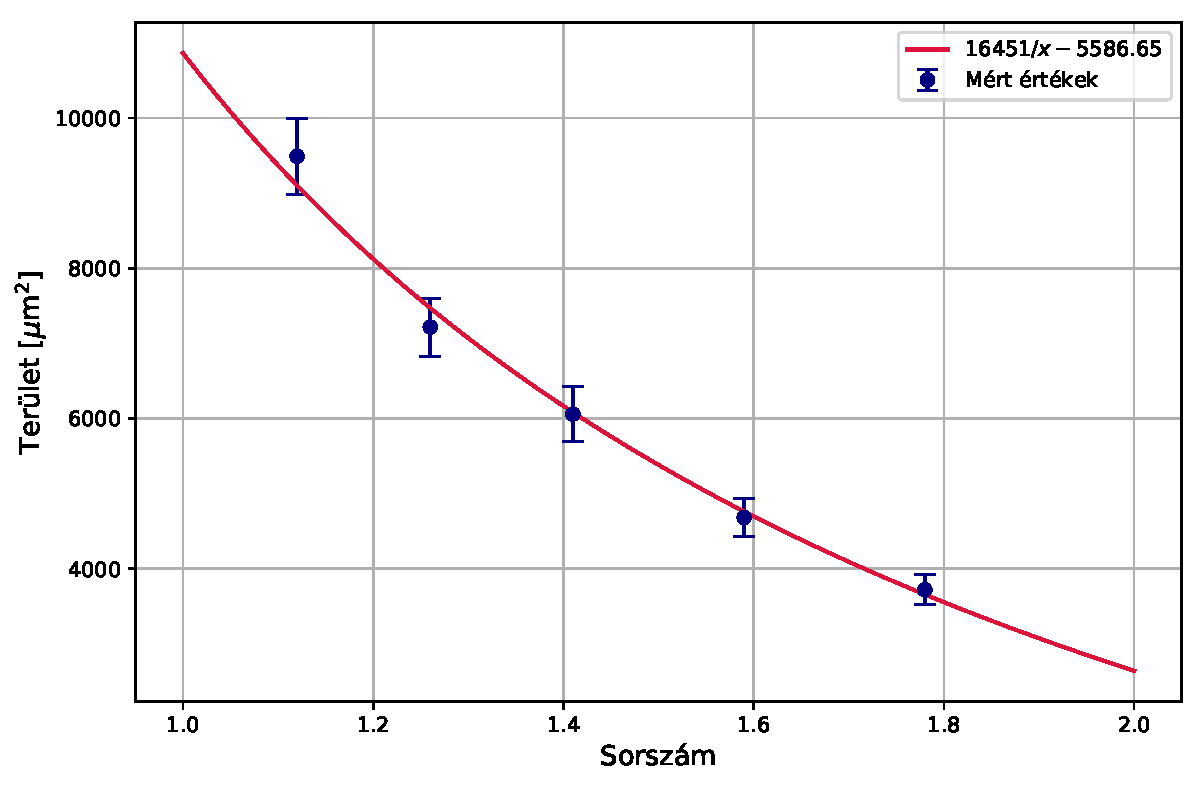
\includegraphics[width=0.8\linewidth]{szil_illesztes}
\caption{A mért értékek illesztésével kapott ábra}
\label{fig:illeszt}
\end{figure}

A fenti ábrán látható, hogy az illesztés hibán belül leírta a megfigyelt változást, vagyis a szilícium mintán látott téglalapok területe és a mellettük látható sorszámok közötti összegfüggés fordított arányosság volt.

\newpage
\section{Légy szemének vizsgálata}
\hspace*{10pt} A mérés során az utolsó feladatként az aranyozott légy szemének vizsgálatát végeztük el különböző nagyításokon. Elsőként 2000x-es nagyításon készítettünk egy képet, mely segítségével aztán meghatároztuk a légy szemén látható cellák átmérőjének nagyságát. A méréshez készült kép a \ref{fig:legy_nagy}. ábrán látható.\\
\begin{figure}[!h]
\centering
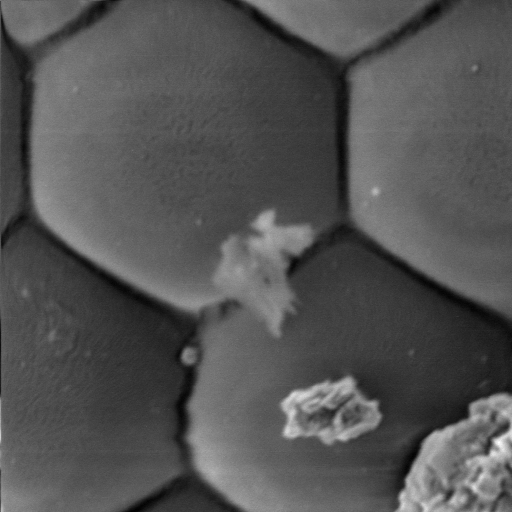
\includegraphics[width=0.8\linewidth]{E/E/014_s}
\caption{A légy szeméről készült 2000x-es nagyítású kép}
\label{fig:legy_nagy}
\end{figure}
\newline
A cella átmérőjének meghatározásához leolvastam két szemközti csúcs pixel koordinátáit, majd kiszámoltam a fizikai méreteket a kalibrációs egyenes segítségével. A kapott cellaátmérő (23.963 $\pm$ 0.705) $\mu$m. A kapott képről emellett a cellák oldalhosszait is meg tudtuk határozni, ehhez csupán a szomszédos csúcsok képen vett távolságát kellett megmérni. A kalibrációs paraméter segítségével kapott átlagos cella oldalhossz: (11.673 $\pm$ 0.642) $\mu$m.\\
\newpage
\hspace*{10pt} Kisebb nagyítás alkalmazása esetén az egyes cellák középpontjai közötti távolságot is megbecsülhetjük. Ehhez lecsökkentettük a nagyítást 700x-ra, majd a \ref{fig:legy_kicsi}. ábrán látható képet készítettük.\\
\begin{figure}[!h]
\centering
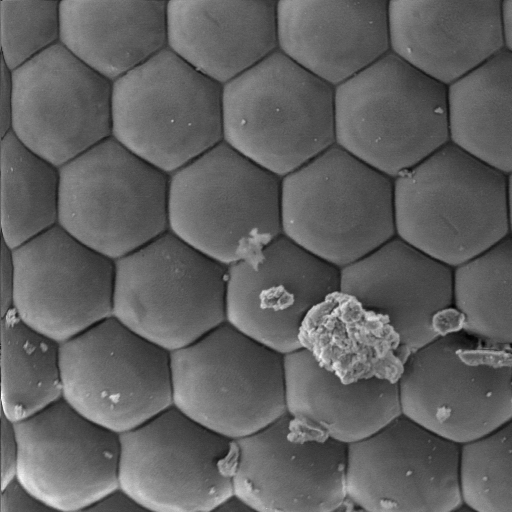
\includegraphics[width=0.8\linewidth]{E/E/015_s}
\caption{A légy szemének 700x-os nagyításon készült képe}
\label{fig:legy_kicsi}
\end{figure}
\newline
A kapott képen kiválasztottam egy cellát, majd a szomszédos hat másik cella középpontjától vett távolságát meghatározva megkaptam a lény szemének rácsparaméterét. A kapott rácsparaméter: (21.764 $\pm$ 1.209) $\mu$m. Ez az érték közel azonos a cella átmérőjének hosszával, vagyis várakozásainknak megfelel.

\section{Diszkusszó}
\hspace*{10pt} Mérésünk során megismerkedtünk a pásztázó elektronmikroszkópia alapjaival, valamint több mintáról készített képet is kiértékeltünk.

\begin{thebibliography}{99}

\bibitem{1} \emph{Kiadott jegyzet}:\\
\texttt{http://metal.elte.hu/oktatas/alkfizlab/meresleirasok/SEM3.pdf}

\end{thebibliography}

\end{document}